% TO-DO:
% * Actions = all possible transtions in RL
% * In RL, Q-learning is still unclear -- currently I'm using NN = transition F(x)
%   -- U(x) -> U(x') so it seems that generalization can occur in Q-space (?)
% * Structure of the turnstile is an important feature of the transition F(x)
% * Explain difference with AIXI
% * "inward" vs "outward"

\documentclass[orivec]{llncs}
\usepackage{graphicx}
\usepackage{amsmath}		% for "cases"
\usepackage{amsfonts}		% for frakur fonts
\usepackage{mathrsfs}		% for curly "E" error symbol
\usepackage{float}
\usepackage[most]{tcolorbox}% for wrapping example in color box
\usepackage{wrapfig}		% wrap figure beside text, used in example
\usepackage{tikz-cd}		% commutative diagrams
% \usepackage{amsfonts}
\usepackage[normalem]{ulem}	% underline with line breaks: /uline
\usepackage{enumitem}       % for using (A),(B),(C) in items...
\usepackage{amssymb}		% for \multimap, \updownarrow, \bigstar
\usepackage{turnstile}		% longer turnstiles
\usepackage{sectsty}		% change section color
\usepackage{hyperref}		% refs, links become clickable
\usepackage{url}			% for urls in bibliography
\usepackage[normalem]{ulem} % underline unbroken with \uline
\usepackage[numbers,sectionbib]{natbib}% if we use \package{url} we need to use natbib style

%\def\chinchin{yes}          % ********** 用中文 *********
% *************** Delete when not using Chinese or colors **********************
\ifdefined\chinchin
	\usepackage{xeCJK}
	\setCJKmainfont[BoldFont=SimHei,ItalicFont=KaiTi]{SimSun}
\fi
\usepackage{color}
%\newcommand{\emp}[1]{\textbf{\textcolor{blue}{#1}}}
\newcommand{\emp}[1]{\textbf{#1}}

\sectionfont{\color{blue}} 
\subsectionfont{\color{blue}} 
\subsubsectionfont{\color{blue}} 
\definecolor{green}{rgb}{0,0.7,0}
\definecolor{grey}{rgb}{0.95,0.95,0.95}

\usepackage{geometry}		% change paper size
\geometry{
  a4paper,         % or letterpaper
  textwidth=18cm,  % llncs has 12.2cm
  textheight=27cm, % llncs has 19.3cm
  heightrounded,   % integer number of lines
  hratio=1:1,      % horizontally centered
  vratio=2:3,      % not vertically centered
}
\usepackage[fontsize=13pt]{scrextend}

\newcommand{\tikzmark}[1]{\tikz[overlay,remember picture] \node (#1) {};}

\newcommand{\vect}[1]{\boldsymbol{#1}}
\newcommand*\sigmoid{\vcenter{\hbox{
\includegraphics{sigmoid.png}}}}
\newcommand*\rectifier{\vcenter{\hbox{\includegraphics{rectifier.png}}}}
\newcommand*\KB{\vcenter{\hbox{
\includegraphics{KB-symbol.png}}}}
\newcommand*\KBsmall{\vcenter{\hbox{\includegraphics{KB-symbol2.png}}}}
\newcommand*\Eye{\vcenter{\hbox{\includegraphics{../eye-symbol.png}}}}
\newcommand*\NN{\vcenter{\hbox{\includegraphics{NN-symbol.png}}}}
\newcommand*\Graph{\vcenter{\hbox{\includegraphics{../graph-symbol.png}}}}
\newcommand*\Hypergraph{\vcenter{\hbox{\includegraphics{../hypergraph-symbol.png}}}}
\newcommand*\Tree{\vcenter{\hbox{\includegraphics{../tree-symbol.png}}}}
\newcommand*\NewSym[1]{\vcenter{\hbox{\includegraphics{#1}}}}
\newcommand{\dashh}{\textemdash~}
\newcommand{\english}[1]{\mbox{\textit{#1}}}
\newcommand{\tab}{\hspace*{2cm}}

% ***** Boxed variables inside math equations
% \newcommand*{\boxedcolor}{black}
\makeatletter
% \renewcommand{\boxed}[1]{\textcolor{\boxedcolor}{%
% \fbox{\normalcolor\m@th$\displaystyle#1$}}}
% \setlength{\fboxsep}{1pt}
\renewcommand{\boxed}[1]{\fbox{\m@th$\displaystyle\scalebox{0.9}{#1}$} \,}
\makeatother

\overfullrule=0mm

\newsavebox{\MyName}
\savebox{\MyName}{
\includegraphics[scale=0.6]{YKY.png}}

\title{
\ifdefined\chinchin
10 分钟介绍强人工智能
\else
10 mins intro to AGI
\fi
}
%\normalsize{-- a minimalist cognitive architecture combining\\
%reinforcement learning and deep learning}}
\titlerunning{}
\author{\usebox{\MyName} (King-Yin Yan)
% \\ \footnotesize{General.Intelligence@Gmail.com}
%\and
%Ben Goertzel
%\and
%Juan Carlos Kuri Pinto
}
\institute{General.Intelligence@Gmail.com}
\date{\today}

\begin{document}
\let\labelitemi\labelitemii

\maketitle

\noindent
\makebox[\linewidth]{\small \today}

\setlength{\parindent}{0em}
\setlength{\parskip}{2.8ex plus0.8ex minus0.8ex}
% \setlength{\parskip}{2.8ex}

\begin{abstract}
\end{abstract}

%\begin{keywords}
%reinforcement learning, control theory, deep learning, cognitive architecture
%\end{keywords}

要研究 AGI,最好熟悉一些 logic-based AI 的基础,这些细节我打算出版一本书叫《强人工智能导论》,正在找合作者写这本书,有兴趣的可以联络。

%\setcounter{section}{-1}
%\section{Bayesian network}
% \label{sec:0}

首先由 Bayesian network 谈起,它是一种命题之间的 graphical model,用以计算某些 nodes 的未知的 probabilities:
\begin{equation}
\vcenter{\hbox{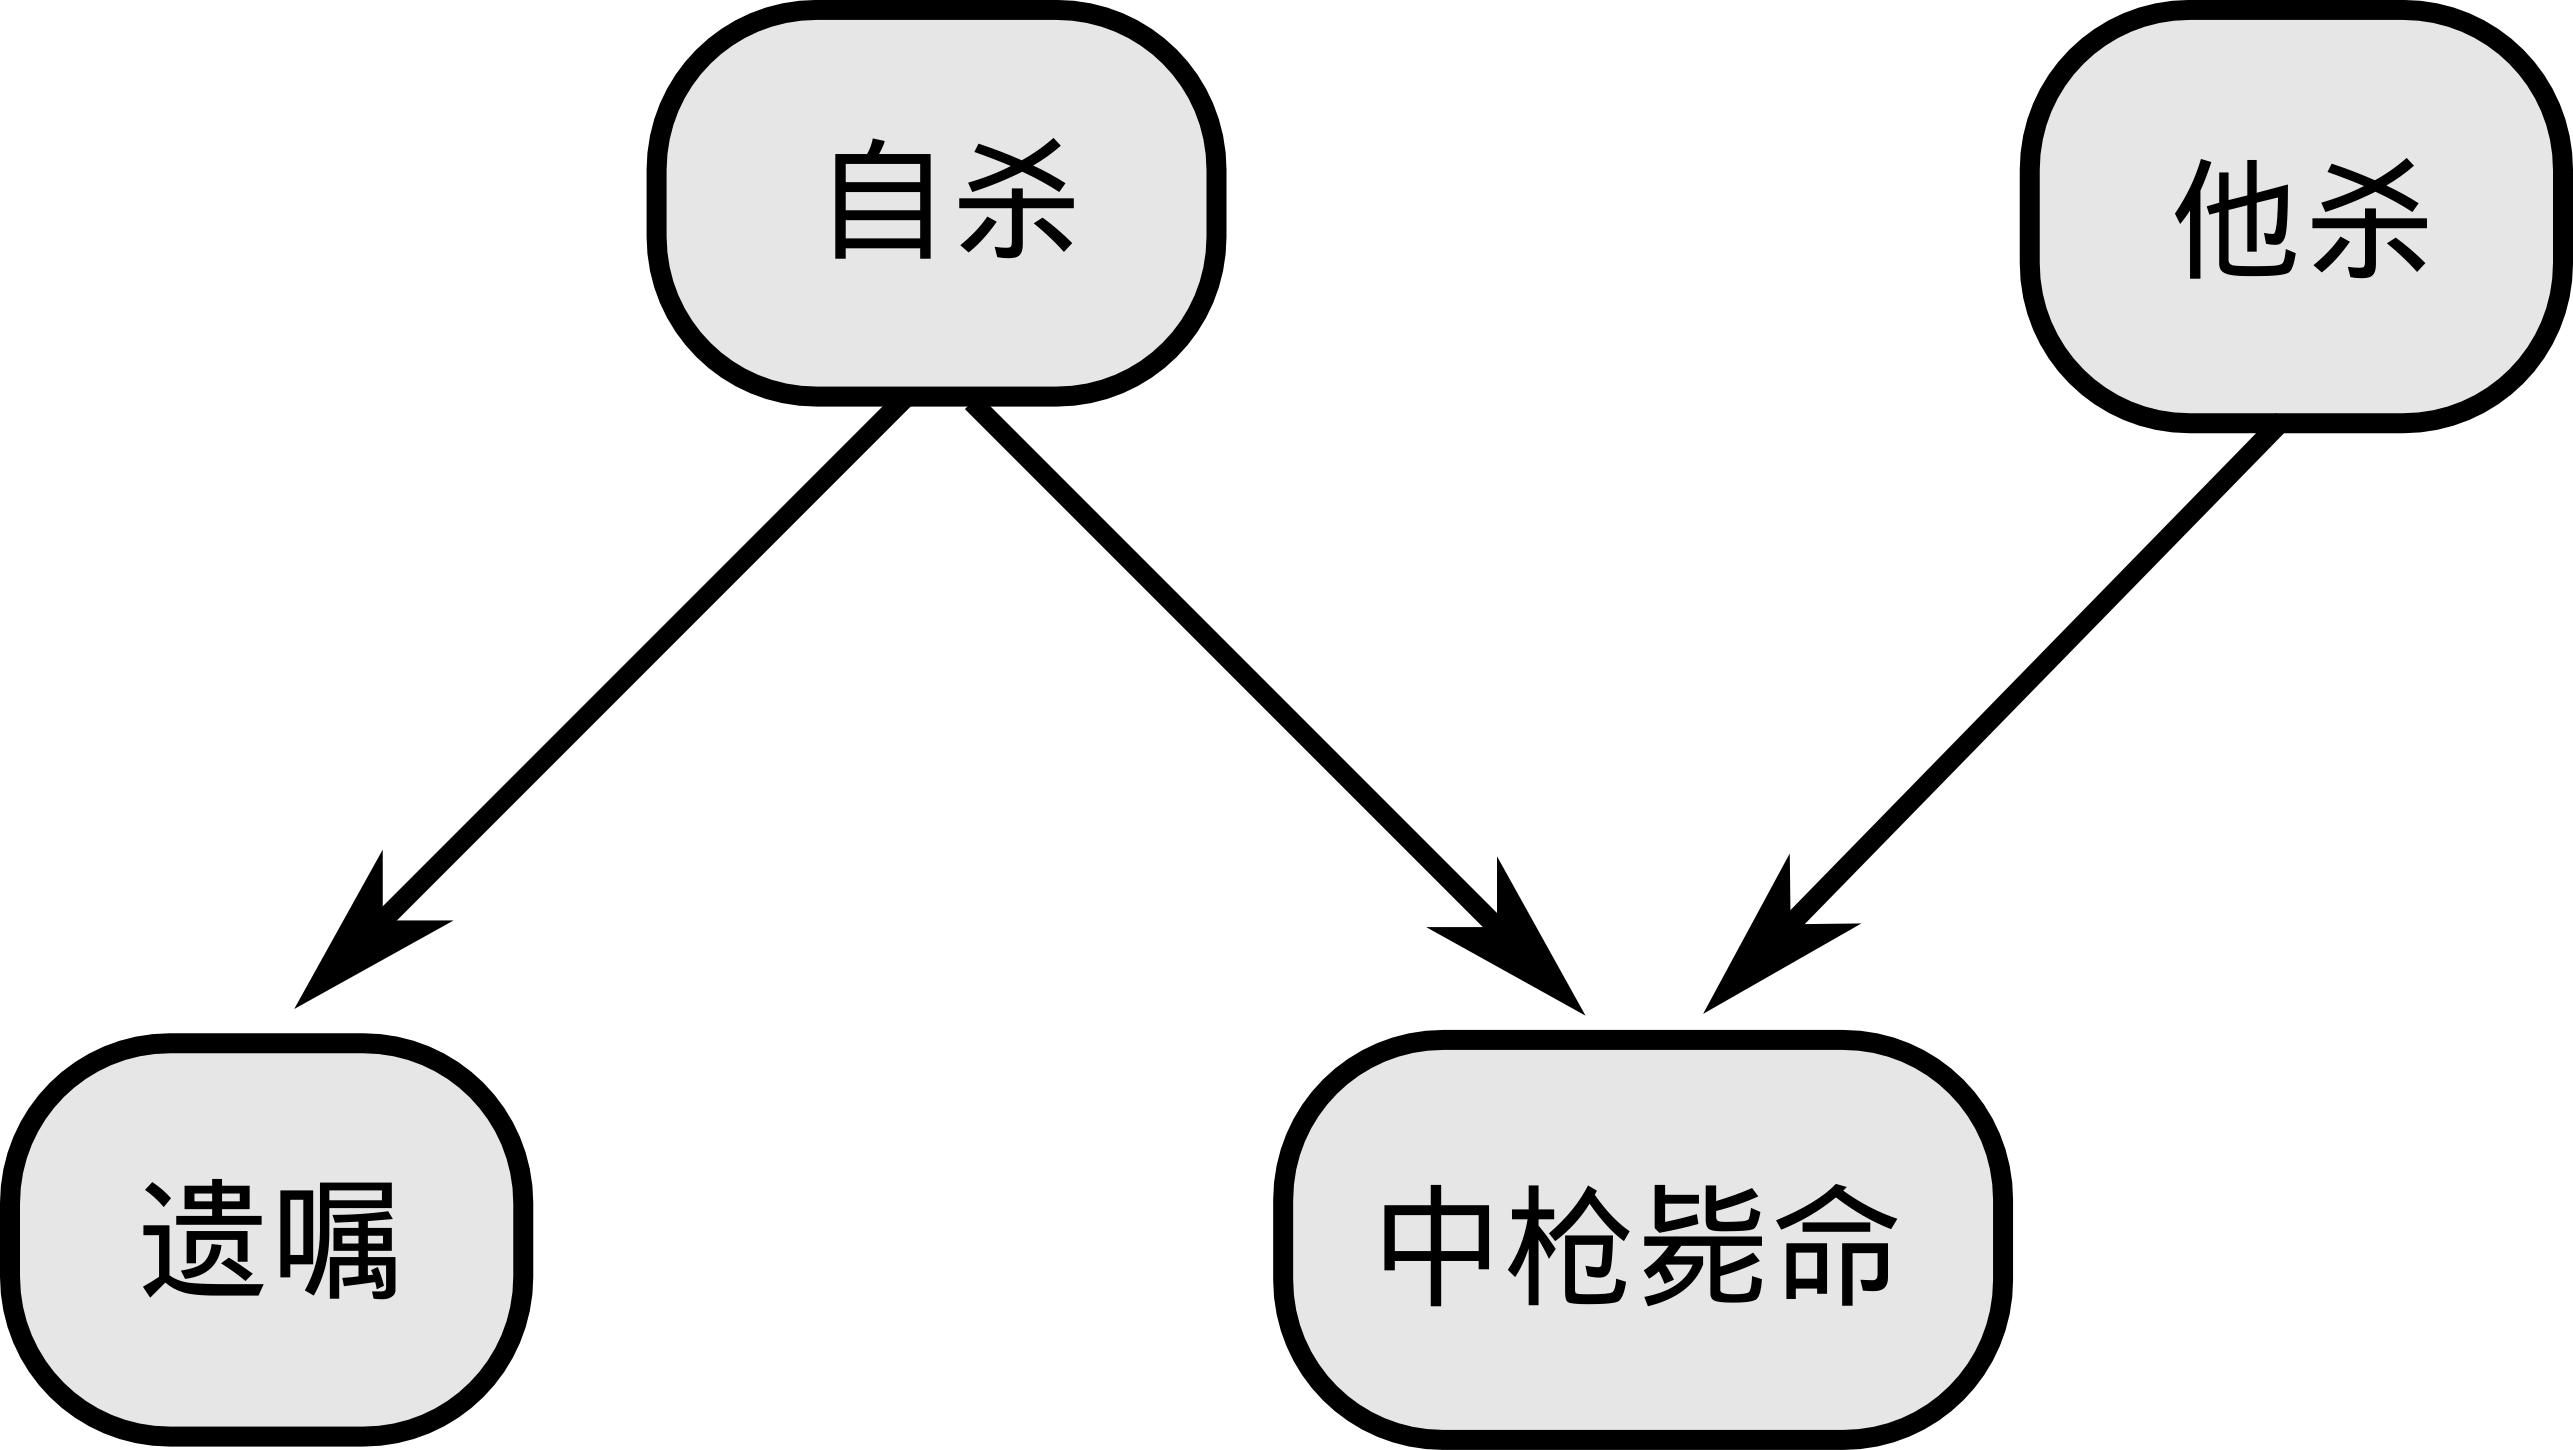
\includegraphics[scale=0.6]{suicide-note.png}}}
\end{equation}

以下的过程叫 ``lifting'':
\begin{equation}
	\boxed{propositional logic} \stackrel{\mbox{lift}}{\longrightarrow} \boxed{Bayesian networks}
\end{equation}

AGI 的其中一个关键步骤是:
\begin{equation}
\boxed{first-order logic} \stackrel{\mbox{lift}}{\longrightarrow} \boxed{first-order Bayesian networks}
\end{equation}
这个问题基本上是可以解决的,其中一个方法叫 KBMC (knowledge-based model construction) :
\begin{equation}
\vcenter{\hbox{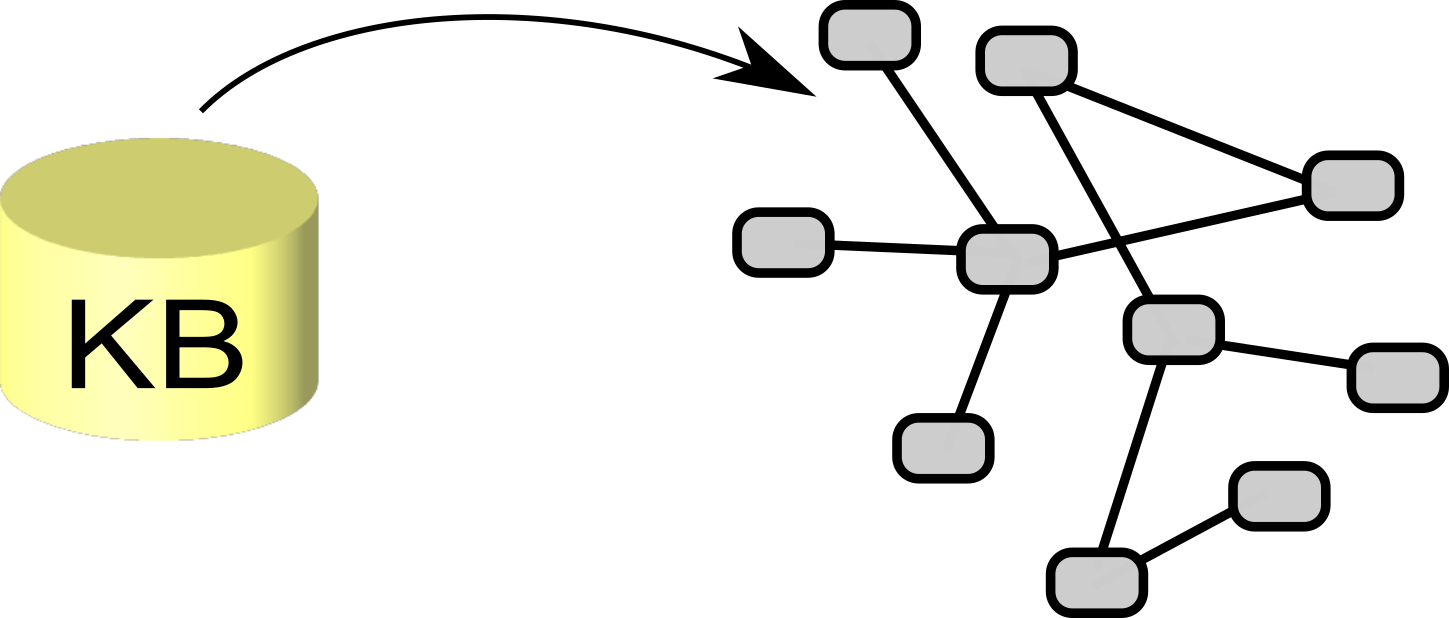
\includegraphics[scale=0.7]{KBMC-illustrated.png}}}
\end{equation}
附带一提,即管在某些名校,如果能做到 lift Bayesian network to probabilistic case,那大概已经可以拿个 PhD,因为这已经算是一种 ``cutting edge'' 的工作(至少在大约 2000-2010 年这段时间,有很多 first-order Bayesian network 的论文出现)。 当然我并没有抵毁 PhD 的意思,但我想指出,在数学上/抽象的角度来看,这其实是一个很简单的动作。 

而且有个更重要的重点:  \uline{这不是瓶颈}。

\underline{\textbf{AGI 的瓶颈是 learning}}。  认识到这一点是非常重要的,AI winter

用 deep learning 模拟 逻辑的 $\vdash$。



\section*{Acknowledgements}

\bibliographystyle{unsrtnat} % or number or aaai ...
\bibliography{AGI-book}

\end{document}
